\documentclass[]{article}
\usepackage{hyperref}
\usepackage{float}
\usepackage[none]{hyphenat}
\usepackage[pdftex]{graphicx}   
\graphicspath{{../pdf/}{../jpeg/}{./image/}}  
\DeclareGraphicsExtensions{.pdf,.jpeg,.png,.jpg} 
%opening
\title{Fact Sheet Link SDGs Challenge}
\author{
	  Eekhout, Wouter\\
	  \texttt{w.t.k.eekhout@fgga.leidenuniv.nl}
	  \and
	  Centre for Innovation\\
	  \texttt{http://www.centre4innovation.org/}
	  \and
	  Leiden Centre of Computer Science\\
	  \texttt{http://lcds.science.leidenuniv.nl/lcds}
	  \and
	  Leiden University\\
	  \texttt{https://www.universiteitleiden.nl/}
}

\begin{document}

\maketitle

\begin{abstract}
This article describes a solution propesed to a challenge by UNDESA/DSD\footnote{\url{https://sustainabledevelopment.un.org/sdg11?page=view&nr=997&type=230&menu=2059}}. 
An open challenge to identify and visualize the relations among the recently adopted sustainable development goals (SDGs) has been launched by the Division for Sustainable Development and Unite Ideas. The challenge consists of building an automated tool that extracts from a set of UN publications all the messages that relate to the relationships between urban development (SDG 11) and all the other SDG areas, and then visualizes the results. 
The solution is online available using: \url{http://linkssdgs.herokuapp.com/}.
\end{abstract}

\section{Introduction/background, problem description}
Sustainable development as an approach tries to understand the world in an integrated, systemic way and focuses on the links among areas. The recently adopted United Nations Sustainable Development Goals (SDGs)\footnote{\url{http://www.un.org/sustainabledevelopment/sustainable-development-goals/}} have defined 17 goal areas, from poverty to oceans to inequality, ecosystems, economic growth, education, etc. Multiple relationships exist among all these goals. A challenge going forward is to better understand them, and map them in a way that is easy to understand while preserving the complexity of the whole. Institutions working on specific areas of sustainable development (e.g. education, energy, slums, etc.) tend to explore and focus on limited aspects of the map. Their policy messages emphasize the importance of specific links. However, for policy discussions, the whole map is needed.

\section{Project description}
The following study provides an overview of the various links between the sustainable development goals throughout key policy documents - with a specific focus on the message that relates to urban development (SDG 11).For this purpose, we have developed an automated classifier to identify how certain texts relate to specific aspects and how these focus areas might be addressed in relation to each other. The classifier has been trained on the basis of the formulation of SDGs and their pertaining targets.

We have provided several visualisations of the classification results with more detailed explanation. Moreover, a demo version of the classification tool. Further information regarding the used approach and methodology behind it can be retrieved through the following link: \url{http://parc.herokuapp.com/file/2014WouterEekhout.pdf}.

The training set and built upon the formulation of the SDG's and their pertaining targets can be found here, while the reports analysed as part of this project can be accessed through the following here: \url{http://bit.ly/LinksSDGsdownload}.

\section{Insights}

\begin{figure}[H]	
	\centering
	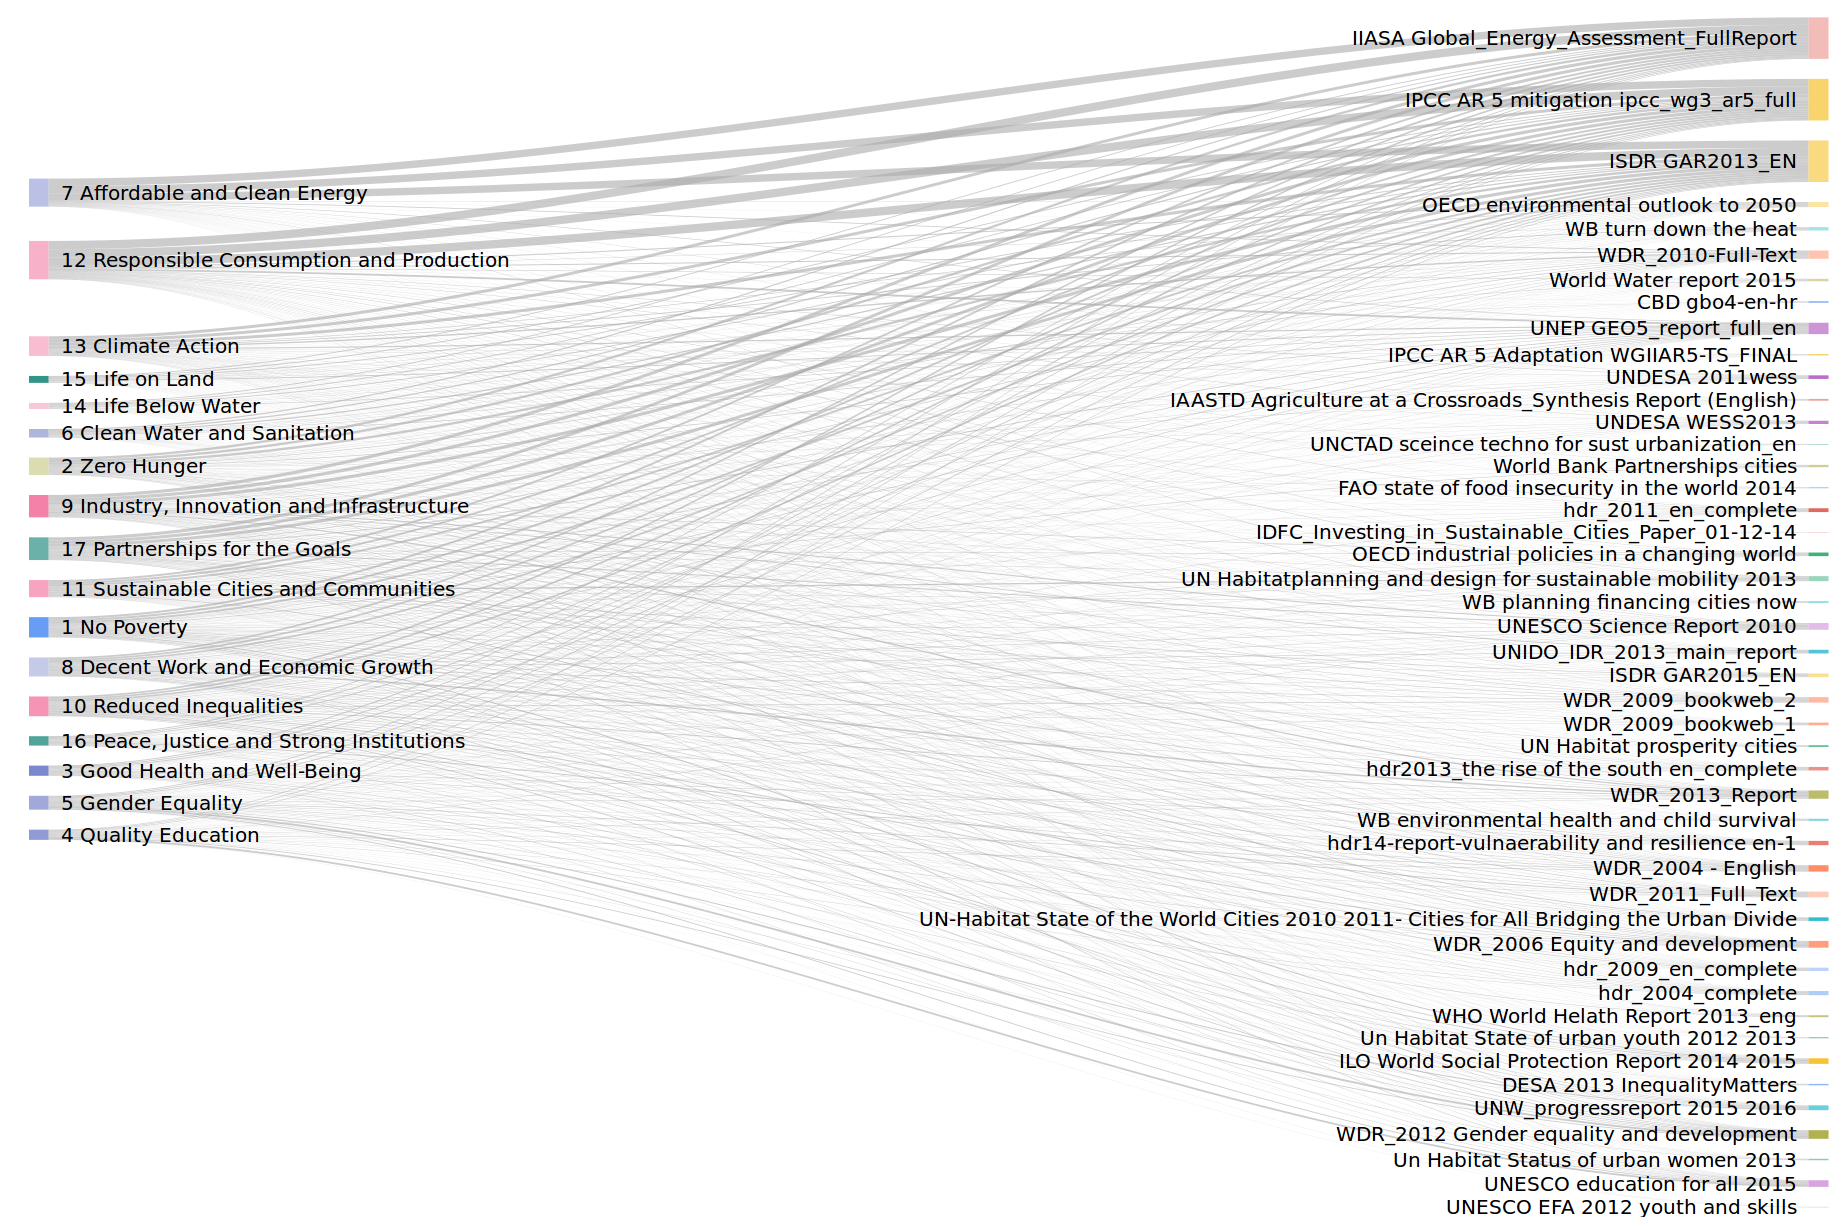
\includegraphics[width=1\textwidth]{Reference_to_SDGs_within_UN_system_flagship_reports.png}
	\caption{Reference to SDGs within UN system flagship reports. Note: The left column represents the SDGs (1-17). The width of each segment is proportional to the amount of texts relating to a specific SDGs within the whole set. The right column features the analysed reports. The width of each segment reflects the absolute amount of texts classified as pertaining to a specific SDG within the specific source. Links from left to right represent the interrelation between a SDG and a specific report. The width of the links is proportional to the number of related messages in each report.}
\end{figure}
\begin{figure}[H]	
	\centering
	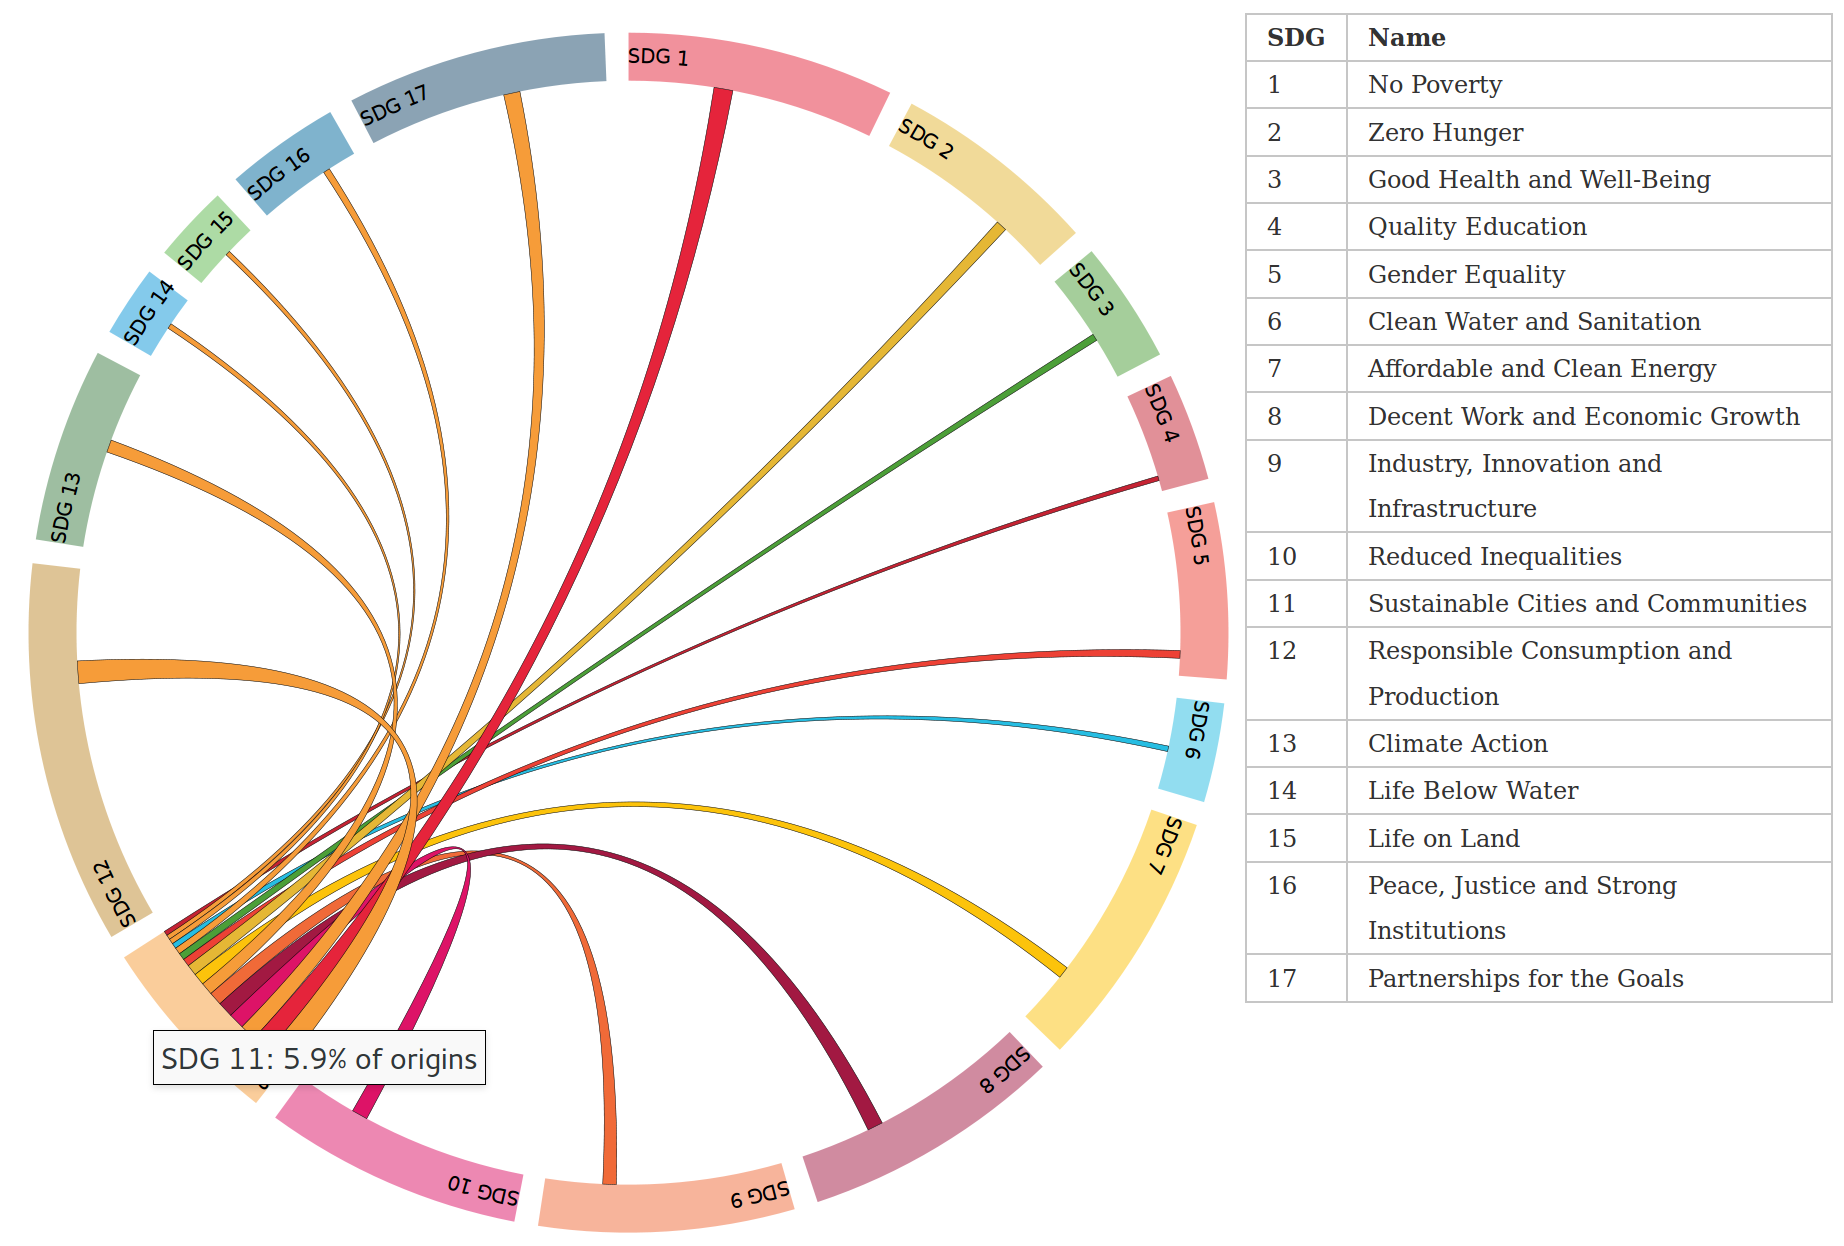
\includegraphics[width=1\textwidth]{Links_between_SDGs_made_within_UN_system_flagship_reports.png}
	\caption{Links between SDGs made within UN system flagship reports. Note: The outer layer of the circle represents the SDGs (1 - 17). The width of each segment is proportional to the amount of texts relating one SDG to another. The lines represent links between two specific SDGs within the whole set. The width of the lines indicates the total amount of texts constituting such links.}
\end{figure}
\begin{figure}[H]	
	\centering
	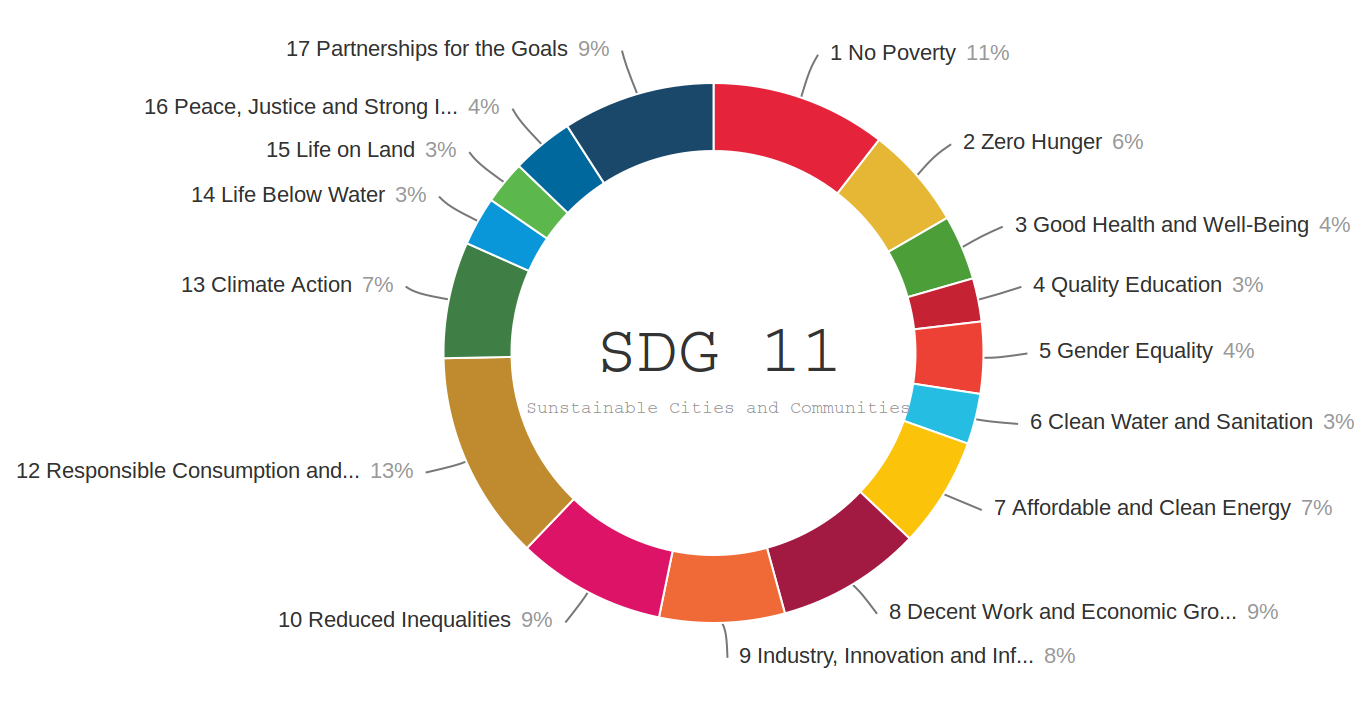
\includegraphics[width=1\textwidth]{Links_between_urban_development_and_other_SDGs_made_within_UN_system_flagship_reports.png}
	\caption{Links between urban development and other SDGs made within UN system flagship reports. Note: The size of each segment represents the total amount of links between the SDG related to urban development (SDG11: ‘Make cities and human settlements inclusive, safe, resilient and sustainable’) and other SDGs within the whole set.}
\end{figure}



\section{Demo tool}
Please try the demo tool out for yourself! The demo is only and is accesible by anyone\footnote{\url{http://linkssdgs.herokuapp.com/index.jsp\#demo_classifier}}. 

An output of the tool is shown in Figure \ref{figure_example_out}. The input is the sentence ``Central to sustainable urban development will be an emphasis on integrated planning in the provision of environmental friendly infrastructure basic services and other public goods''. The results are classified per sentence. The bar chart shows the total sum of all the categories of the provided text. For the example sentence the prediction is label 11 and 9. When clicking on the link ``Show info'', more inside information is shown.

\begin{figure}[!ht]\label{figure_example_out}
	\centering
	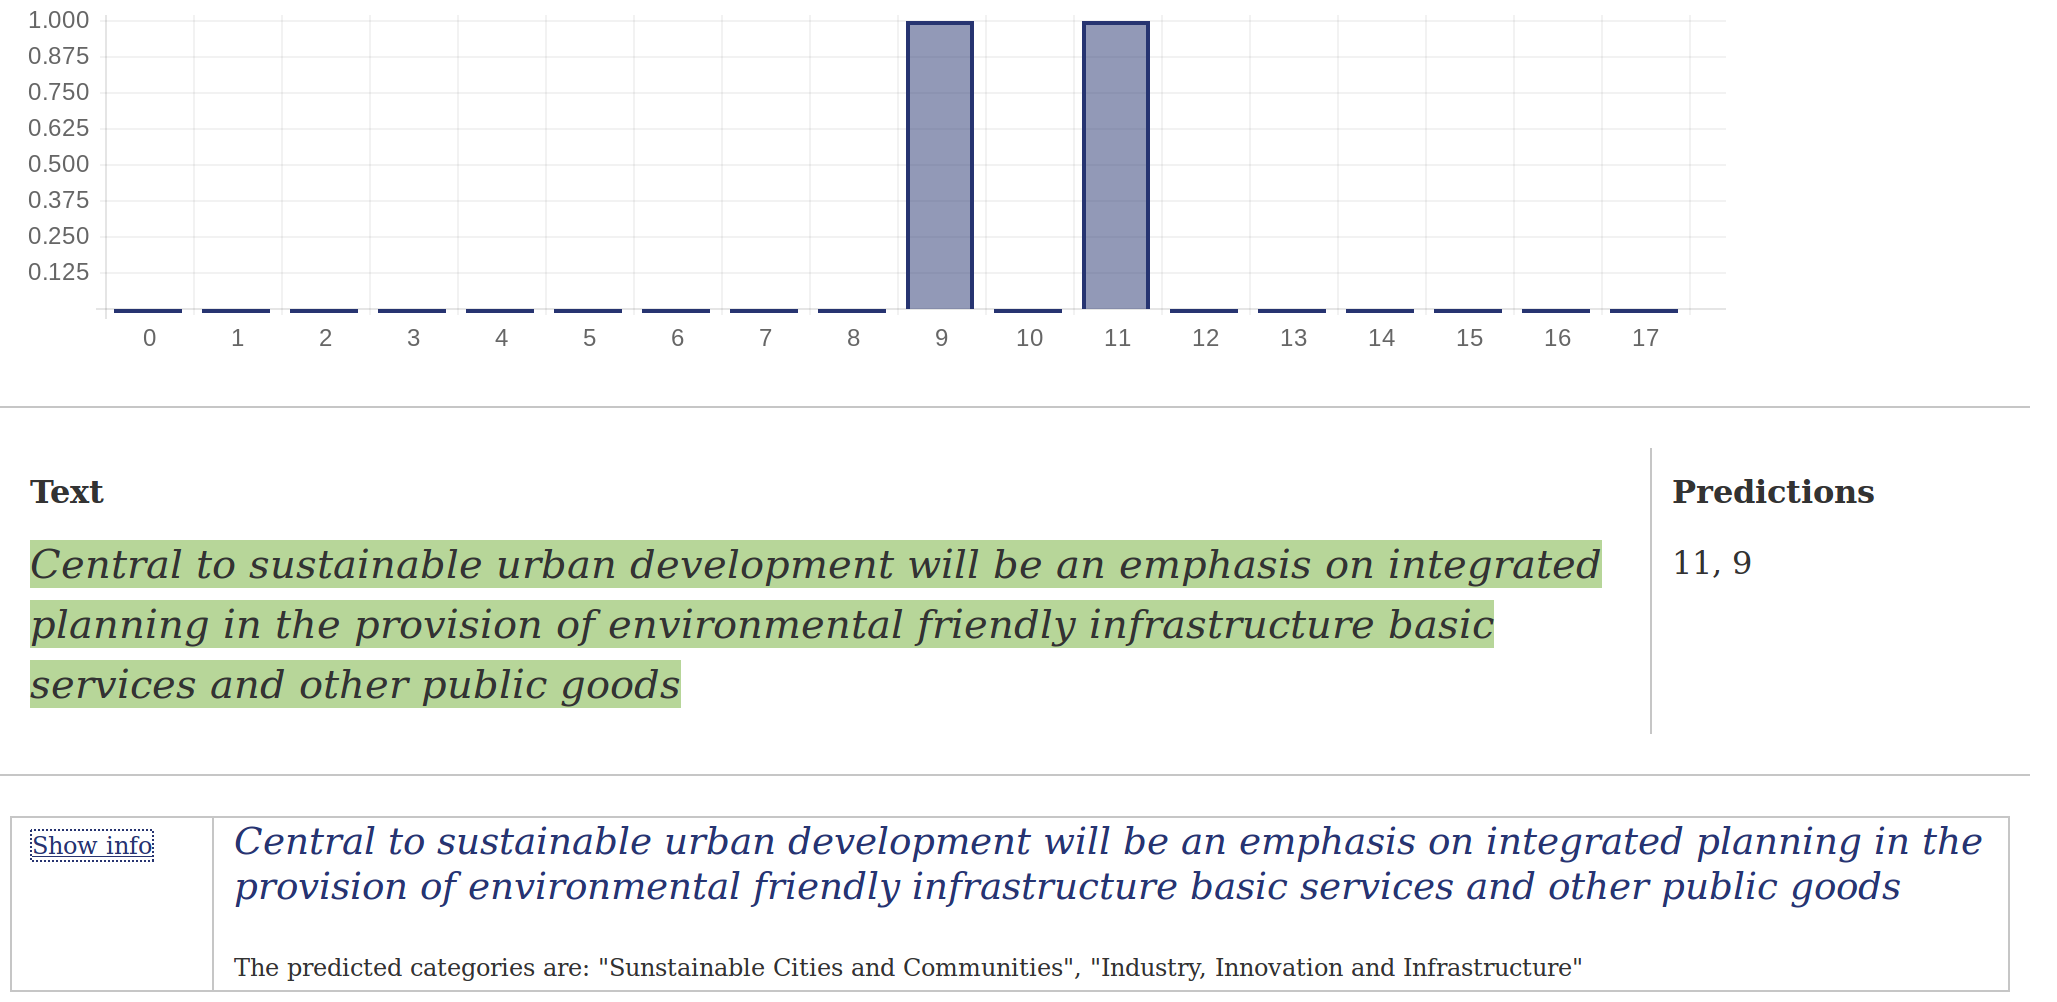
\includegraphics[width=1\textwidth]{example_output.png}
	\caption{Example out of the demo tool for the sentence: ``Central to sustainable urban development will be an emphasis on integrated planning in the provision of environmental friendly infrastructure basic services and other public goods.''}
\end{figure}

\section{Conclusions: opportunities and challenges}
The classifier works well on classifying large documents. This makes it easier to create insights in a short period. For instance decision making on which documents to focus. Also the classifier can be used real time, for i.e. classifying Tweets from Twitter. A real time solution can be made to see about which SDG's are tweeted the most. 

Another use can be to pre-classify huge amount of text and a person later validating the results. This greatly reduces the time needed to classify huge amounts of text. Especially when two or more person are classifying the same text in order to maintain a certain quality and validity in the final product. This way of working is being used for classifying Dutch documents in political categories\footnote{\url{http://parc.herokuapp.com}} with the same classifier as described in this article.  

\section{How to move forward}
The next steps are to further improve the classifier. The classifier needs extra trained data to improve the outcome of the classifier. This can be done real-time in the form of an feedback loop. Where a user corrects the outcome and the classifier and the classifiers learns from the user. This is the way in which classifiers stay up to date with the current change, this can be done real time.

\end{document}
            
